\documentclass{article}
\usepackage[utf8]{inputenc}
\usepackage{minted}
\setminted{fontsize=\small}
\usepackage{multicol}
\newmintinline[Li]{Lua}{}
\newmintinline[Ci]{C}{}
\usepackage{pgfplots}
\pgfplotsset{compat=1.14}

\title{Current Progress on XTask, from the 2017 BigDataX REU}
\author{Jonathon Anderson, aka blue42u}
\date{July 2017}

\begin{document}

\maketitle

\section{Introduction}
In recent years, the importance of parallelism has grown significantly, in no small part thanks to the development into multi- and many-core processors. While this is very convenient for computation, actually fully utilizing all of those processors is often difficult for processes that are not already embarrassingly parallel. To make matters worse, writing parallel code is often difficult for less experienced programmers, and the plethora of languages designed to fix that have had the side effect of segregating the community into smaller user groups.

In another vein, we also have the theoretical solution to deal with. If we could remove the overhead from context switches and synchronization, we could split any code up into a bunch of single instructions with dependencies, and then run them in parallel (as much as possible). In practice, this is an unfeasible solution, since the overhead incurred is in fact quite large. In cases where the entire graph is available early on (or at the very least its general shape is determinable) this can be mitigated by deciding the distribution early, but that is not possible with many interpreted languages.

The XTask project aims to aid in solving both of these issues. The main goal is to provide a runtime (and thus dynamic) system for processing many extremely small tasks at reasonable speeds, but compile-time systems like Cilk and OpenMP are far faster than anything a dynamic system can do. Thus rather than comparing on that level, XTask's main use case now is in interpreters, and (in the large picture) aims to aid such systems with a powerful threading scheme, closing the gap once again between the compiled and interpreted languages.

That is where XTask is now. Of course, everything has to start somewhere.

\section{Short History}
XTask started off, like most things, without the directions of becoming a key part to the software community. Rather it started off as a research project to try and find the fastest multi-producer and -consumer queue, for the purposes of building a threaded interpreter for the dataflow language Swift/T. The Swift project had already been running into performance issues with small tasks, and so the main goal was to adapt the interpreter to use a threaded model instead of MPI, although the obvious cost would be the loss of multi-node processing. If properly adapted, that would be added back in later.

Unfortunately for that goal, after about 3 weeks of preliminary experimentation within the Swift/T engine, it became clear that the entire engine would need an overhaul before a threaded system would be viable. There were two main reasons, one being that Swift/T's VM, Turbine, was designed from day one to use MPI, and as such uses a multi-process model rather than a multi-threaded model. This would make the adaption process difficult to progress, as every global and every execution path would have had to be carefully traced out and made safe. The second reason was that Swift/T's compiler to its VM did not perform any compile-time analysis of the dependency graph, and for speed we decided that XTask would not fill that role (essentially pushing graph-theoretic algorithms into the application).

As such, the goal of being able to use existing Swift code to test XTask was postponed, replacing it instead with the development and refinement of a separate API. This API went through about 3 iterations (which means there's room for improvement) before achieving the state at which it stands at the time of this writing, but it was during that development that the two goals mentioned before came to light as the perfect niche to fit XTask into. The API is designed using a powerful but small paradigm that was developed in tandem as various benchmarks were written and the results compared.

It is this paradigm that give XTask's API its potential to achieve its goals.

\section{The Paradigm}
The paradigm behind XTask can be formulated as a short list of statements, most succinctly worded as the following:
\begin{enumerate}
    \item ``Tasks'' are invocations (running and planned) of functions with user-defined data.
    \item One Task may depend on another Task, thus ordering the executions of the tasks, as well as creating a dependency graph.
    \item After execution, a Task has a choice between ``leafing'' which removes itself from the dependency graph and may allow other Tasks to run...
    \item ...or ``tailing``, which replaces itself with the last-executed Tasks of a smaller dependency graph.
    \item At any given point in time, the dependency graph must form a tree where the children of any Task must complete before their parent Task.
\end{enumerate}
This is analogous to a language in which all function invocations (1) are able to run in parallel, and return values are properly transferred between the functions (2), but calls to a function can only occur as part of the return value (3,4), and there are no variables (5).

Interestingly enough, it turns out that the last two ``issues'' with our pseudo-language are actually easy to fix, the first with a subdivision of what most languages consider ``functions'', and the second with a little graph theory. The XTask interface layer does neither of these (nor should it), and it is up to higher layers and applications to perform these tasks, either at parse/compile time or at runtime (if possible).

\subsection{A Simple Example}
It might be a little hard to see why this is sufficient (and a bit refreshing), but hopefully a few examples will prove convincing. Suppose we have a fairly ordinary implicitly parallel language, with some code like so:
\begin{minted}{Lua}
function f1()
    x = g()
    y = h()
    return x + y
end
\end{minted}
In dataflow schemes, this would be translated by the interpreter into a single thread's code, as something like
\begin{minted}{C}
var o f1() {
    var x, y;
    spawn_thread x g();
    spawn_thread y h();
    spawn_thread o __add x y;
}
\end{minted}
However, XTask doesn't support spawning new tasks during a task's execution. Its not hard to translate the original though, and the result is something like
\begin{minted}{Lua}
function f1()
    return __add(g(), h())
end
\end{minted}
In other words, once \Li{f1} completes \textit{any task that was waiting for its completion will now be waiting on the completion of \Li{__add}, which in turn is waiting on the completion of \Li{g} and \Li{h}}, assuming that data motion is mapped accordingly to task dependencies.

\subsection{Fork-join Style}
Its also pretty easy to perform fork-join styled processing without too much difference, although the function does need divided into pieces. Again in the implicitly parallel language:
\begin{minted}{Lua}
function f2()
    -- Stuff before...
    for i = 1,n do
        -- Stuff in threads...
    end
    -- Stuff after...
end
\end{minted}
The \Li{for} loop is done in parallel, so each ``thread'' of the loop will become a separate task, and the stuff after will depend on the stuff in the threads. Thus it can be translated into something like:
\begin{minted}{Lua}
function f2()
    -- Stuff before...
    return after(inner(1), inner(2), ..., inner(n))
end
function inner(i)
    -- Stuff in threads...
end
function after(...)
    -- Stuff after...
end
\end{minted}
Of course, this assumes that the number of arguments is dynamic or can be ignored, and a proper implementation may instead use some sort of array structure to hold the (possibly large) number of tasks.

\subsection{Variables}
As far as dataflow-styled constructs go, the only other interesting examples come from the use of variables. Its a bit more sticky than the fork-join scheme, and requires a bit of graph theory to perform properly, but is still fairly easy. Let's use the following as an example.
\begin{minted}{Lua}
function f3()
    x = g()
    return h(x) + k(x)
end
\end{minted}
The issue here is that our paradigm only allows for one task to depend on \Li{g}, but here both \Li{h} and \Li{k} do. The solution to this is to again split up the function, like so
\begin{minted}{Lua}
function f3()
    return hk(g())
end
function hk(x)
    return h(x) + k(x)
end
\end{minted}
In other terms, the technique is to use the execution of a task for synchronization, rather than a normal task dependency. The obvious downside is that one extra tasks is needed to fit the paradigm, although the execution of the task is also extremely small.

It turns out that moving these little managerial tasks to higher layers is very beneficial for the system as a whole.

\section{The API Design}
Since the interface layer is the only other source of overhead besides the dispatching implementation itself, care was taken to ensure that this layer was as thin as possible, and does very little work of its own. While the API follows the paradigm closely, there are a handful of design decisions that were made as more and more benchmarks were run, which are not insignificant parts of the research. Because of this, we will go through the current API and describe how it works as an implementation of the paradigm.

First, we should describe what a task looks like. It should be noted that XTask does not do any memory management for the tasks\footnote{The reason for this is due to a discovery during the benchmarks that often much of the time was spent performing the many \Ci{malloc}s and \Ci{free}s. The next iteration of the API fixed this by forcing the application to manage its own memory, which it could do far better than XTask could.}, which allows for the application to build custom structures that contain both XTask task data and application task data. As such, all references to tasks in the XTask API are \Ci{void*}, which is assumed to point to a structure who's first member is an \Ci{xtask_task}, defined as follows:
\begin{minted}{C}
typedef struct {
    xtask_taskfunc func;
    int fate;
    void* children;
    void* sibling;
} xtask_task;
\end{minted}
In this structure, \Ci{func} and \Ci{fate} define and describe the execution of the task itself, while \Ci{children} and \Ci{sibling} form the pointers of the tree of tasks required by the paradigm. In particular, the \Ci{sibling} members form a linked list between the children of a single node, while the \Ci{children} member points to the head of that list. For future use, \Ci{fate} is a bitmask that can give hints to the runtime as to what \Ci{func} expects or will return, the only allowed values so far being \Ci{0} or \Ci{XTASK_FATE_LEAF}, which indicates whether it is certain to leaf or not. As an example, Figure \ref{fig:memory} shows a small task-tree.

\begin{figure}
    \centering
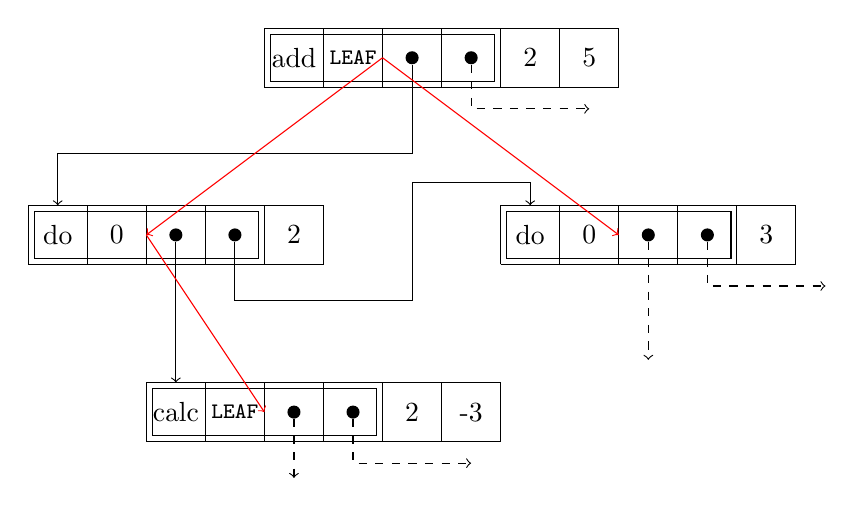
\begin{tikzpicture}[scale=.75]

\begin{scope}[shift={(0,0)}]
\coordinate (A) at (-2.5,1);
\coordinate (Ak) at (-1,.5);
\draw (-3,0) grid (3,1);
\draw (-2.9,.1) rectangle (.9,.9);
\node at (-2.5,.5) {add};
\node at (-1.5,.5) {\footnotesize\texttt{LEAF}};
\node[circle,fill=black,scale=.5] (Ac) at (-0.5,.5) {};
\node[circle,fill=black,scale=.5] (As) at (0.5,.5) {};
\node at (1.5,.5) {2};
\node at (2.5,.5) {5};
\end{scope}

\begin{scope}[shift={(-4,-3)}]
\coordinate (B) at (-2.5,1);
\coordinate (Bk) at (-1,.5);
\draw (-3,0) grid (2,1);
\draw (-2.9,.1) rectangle (.9,.9);
\node at (-2.5,.5) {do};
\node at (-1.5,.5) {0};
\node[circle,fill=black,scale=.5] (Bc) at (-0.5,.5) {};
\node[circle,fill=black,scale=.5] (Bs) at (0.5,.5) {};
\node at (1.5,.5) {2};
\end{scope}

\begin{scope}[shift={(4,-3)}]
\coordinate (C) at (-2.5,1);
\coordinate (Ck) at (-1,.5);
\draw (-3,0) grid (2,1);
\draw (-2.9,.1) rectangle (.9,.9);
\node at (-2.5,.5) {do};
\node at (-1.5,.5) {0};
\node[circle,fill=black,scale=.5] (Cc) at (-0.5,.5) {};
\node[circle,fill=black,scale=.5] (Cs) at (0.5,.5) {};
\node at (1.5,.5) {3};
\end{scope}

\begin{scope}[shift={(-2,-6)}]
\coordinate (D) at (-2.5,1);
\coordinate (Dk) at (-1,.5);
\draw (-3,0) grid (3,1);
\draw (-2.9,.1) rectangle (.9,.9);
\node at (-2.5,.5) {calc};
\node at (-1.5,.5) {\footnotesize\texttt{LEAF}};
\node[circle,fill=black,scale=.5] (Dc) at (-0.5,.5) {};
\node[circle,fill=black,scale=.5] (Ds) at (0.5,.5) {};
\node at (1.5,.5) {2};
\node at (2.5,.5) {-3};
\end{scope}

\draw[->] (Ac.south) -- +(0,-1.5) -| (B.north);
\draw[->,dashed] (As.south) |- +(2,-.75);
\draw[->] (Bc.south) -- +(0,-1.5) -| (D.north);
\draw[->] (Bs.south) -- +(0,-1) -| +(3,1) -| (C.north);
\draw[->,dashed] (Cs.south) |- +(2,-.75);
\draw[->,dashed] (Cc.south) -- +(0,-2);
\draw[->,dashed] (Ds.south) |- +(2,-.75);
\draw[->,dashed] (Dc.south) -- +(0,-1);

\draw[->,red] (Ak) -- (Bk);
\draw[->,red] (Bk) -- (Dk);
\draw[->,red] (Ak) -- (Ck);

    \end{tikzpicture}
    \caption{An example small task-tree. The red edges shows the tree's edges, the double-boxed members are part of the \Ci{xtask_task} structure, and the black arrows show the locations of pointers.}
    \label{fig:memory}
\end{figure}

%\pagebreak

Of course, to execute a task there needs to be a function for XTask to call, so the functions used as values for the \Ci{func} member have the following signature:
\mint{C}{void* func(void* state, void* task);}
The first of the two arguments points to some application-defined ``state'', which during the execution of \Ci{func}, is guaranteed to be unique. That is, while \Ci{func} is running, no other task will be executing with the same \Ci{state}.\footnote{Internally this is currently implemented using a \Ci{void*} on the thread's stack.} The second argument points to the task structure that is being executed, which allows the invocation access to the application-defined structure. The return value is a pointer to the root of the task-tree that the task will tail into (with the effects described above), and can be \Ci{NULL} to indicate leafing.

The final component of the XTask API is a single function that synchronously runs a task-tree. The signature is as follows:
\mint{C}{void xtask_run(void* task, xtask_config cfg);}
Where \Ci{task} points to the root of the task-tree to execute, and \Ci{cfg} is a structure that contains information on the number of workers to use, and creation and destruction function pointers for the \Ci{state}s. This function, when called, will spawn the threads and insert the given task-tree for execution, waiting for it to complete \textit{including modifications made by tailing} before returning.

Of course, an API is only as good as its usefulness. We wrote some extensions on top of XTask just to be sure that generality was actually achieved.

\section{Extensions}
There are two extensions to XTask that have been written, although neither of them are currently able to handle every case that they should. They both would perform the graph theory necessary to properly handle variables (as before), but that has not yet been implemented.

\subsection{XData}
The first extension is XData, which provides a dataflow-styled interface rather than the normal task-tree interface from XTask. The idea is that every task will take in a number of inputs, and output a single value that can then be used by other tasks. The API itself has not gone through all of the development it would need for a production system, so here we present only a sample of code written using the macros provided as part of the interface:

%\pagebreak

\begin{minted}{C}
#include <xdata.h>

static xd_F(add, dummy, in) {
    int *a = in[0], *b = in[1];     // The inputs are provided as an array of void*.
    xd_O(int, *a + *b);             // xd_O sets the output to a given constant.
}

static xd_F(fib, dummy, in) {
    int *n = in[0];                 // It is assumed the type and number of inputs is constant.

    if(*n <= 1) xd_O(int, *n);
    else {
        xd_C(int, a);               // xd_C creates a new line (variable to transfer data with).
        xd_CV(int, an, *n-1);       // xd_CV is the same, but also sets its value.
        xd_P(a, fib, an);           // xd_P "prepares" a task, with the given inputs and output.
                                    // The following are equivalent statements in a dataflow language.
        xd_C(int, b);               // int b;
        xd_CV(int, bn, *n-2);       // int bn = n-2;
        xd_P(b, fib, bn);           // b = fib(bn);
                                    // The output line is accessable from the XD_OUT macro.
        xd_P(XD_OUT, add, a, b);    // out = add(a, b);
    }
}

int main(int argc, char** argv) {
    xtask_config xc = { .workers=5, };      // All this is setup...
    int fibindex = 30;
    int out;

    xd_R(xc, &out, fib, &fibindex);         // xd_R is like xd_P, but for the main thread.

    printf("%d\n", out);
    return 0;
}
\end{minted}

\subsection{Lua}
The other extension on top of XTask is a binding for Lua. Lua is a full-fledged scripting language, so while this shows that the XTask API is flexible enough to perform the role it intends to fill, it is slower than C (about 2-3x on benchmarks that are not based around string operations). The language is far easier to write in, the binding consisting of a single function \Li{defer}, which ``defers'' a call to a function and as such returns a ``Deferred'' object. By treating this object as a function and calling it, the function will run (if not in a task) and return once the function completes. Again, we provide only an example:

%\pagebreak

\begin{minted}{Lua}
require 'xtask'

local function add(a, b)    -- Addition is not implicitly handled, so we do it ourselves.
    return a + b
end

local function f(n)
    if n <= 1 then return n -- Deferred calls gain dependencies from Deferred arguments
    else return defer(add, defer(f, n-1), defer(f, n-2)) end 
end

print( defer(f, 30)({workers=5}) )  -- Calling a Deferred returns the result of the call
\end{minted}

\section{Results}
Throughout the development of XTask, a constant side branch of the research was designing and performing benchmarks on multiple systems that are comparable to XTask in one way or another. By the time of this writing, there were five benchmarks that were written, although only four were used. These are:
\begin{itemize}
    \item A stress test, where the tasks are empty and so the only time taken is by the function call and the task managment itself.
    \item A recursive Fibonacci calculation, so each task consists of a branch and a few additions.
    \item A nested for loop, which was converted from a physics application, and
    \item An implementation of the classic Quicksort, which has a nice range of tasks reducing in size as the process progresses.
\end{itemize}
The fifth unused benchmark was did some matrix operations, but unfortunately the different systems would treat it slightly differently and cause the data to not match up with the other results. The final graphs for the current implementation of XTask can be seen in Figure \ref{fig:graphs}. In general, XTask clocks in at about 100x slower than equivalent C code, although this number could probably be improved with more development.

\begin{figure}
\pgfplotsset{every axis/.append style={
    ymajorgrids=true, grid style=dashed,
    xtick distance=6, xtickmin=0, xtickmax=48,
}}
\centering
\hspace*{-18ex}
\begin{tikzpicture}[font=\small]
\matrix{
\begin{semilogyaxis}[ylabel={Tasks/Sec}]
\addplot[mark=none,color=purple]     table[x=Threads,y=TPS] {chi/nap-single.dat};
\addplot[mark=none,color=red]        table[x=Threads,y=TPS] {chi/nap-cilk.dat};
\addplot[mark=none,color=blue]       table[x=Threads,y=TPS] {chi/nap-jigstack.dat};
%\addplot[mark=none,color=blue!40!green]       table[x=Threads,y=TPS] {chi/nap-jigstackxd.dat};
\addplot[mark=none,color=black]      table[x=Threads,y=TPS] {chi/nap-swiftt.dat};
\end{semilogyaxis}
&
\begin{semilogyaxis}[legend to name=legend, legend columns=-1]
\addplot[mark=none,color=purple]     table[x=Threads,y=TPS] {chi/fib-single.dat};
\addplot[mark=none,color=red]        table[x=Threads,y=TPS] {chi/fib-cilk.dat};
\addplot[mark=none,color=blue]       table[x=Threads,y=TPS] {chi/fib-jigstack.dat};
\addplot[mark=none,color=blue!80!green]       table[x=Threads,y=TPS] {chi/fib-jigstackxd.dat};
\addplot[mark=none,color=blue!40!green]       table[x=Threads,y=TPS] {chi/fib-xtasklua.dat};
\addplot[mark=none,color=black]      table[x=Threads,y=TPS] {chi/fib-swiftt.dat};
\legend{Single, Cilk, XTask, XData, Lua, Swift/T};
\end{semilogyaxis}
\\
\begin{semilogyaxis}[ylabel={Tasks/Sec}, xlabel={Threads}]
\addplot[mark=none,color=purple]     table[x=Threads,y=TPS] {chi/mdlite-single.dat};
\addplot[mark=none,color=blue]       table[x=Threads,y=TPS] {chi/mdlite-jigstack.dat};
\end{semilogyaxis}
&
\begin{semilogyaxis}[xlabel={Threads}]
\addplot[mark=none,color=purple]     table[x=Threads,y=TPS] {chi/qsort-single.dat};
\addplot[mark=none,color=red]        table[x=Threads,y=TPS] {chi/qsort-cilk.dat};
\addplot[mark=none,color=blue]       table[x=Threads,y=TPS] {chi/qsort-jigstack.dat};
\end{semilogyaxis}
\\
};
\end{tikzpicture}
\ref{legend}
\caption{The final round of data from the benchmarks. All tests were run on a 2-CPU, 48-thread system provided by the Chameleon Cloud. The drops in XTask performance after 24 threads are due to hammering of the cache, since the system is not as of yet NUMA-aware.}
\label{fig:graphs}
\end{figure}

%\pagebreak

\section{Conclusion and Future}
We have managed to construct a dynamic API that is capable of achieving comparable speeds when compared to raw C code, while still preserving the flexibility needed for dynamic languages. While we have not yet achieved the original goals of the project, this provides a significant step forward towards both them, and brings the compiled vs. interpreted language wars into the parallel realm.

There are still many goals that XTask will need to reach before its conclusion, and of course we have many ideas as to various tasks that can be done along the way. Here are listed a few of the more exciting ones.
\begin{itemize}
    \item Rebuild the internal dispatcher to fully use the prior research, giving the system a significant boost in performance (if the preliminary tests are to be trusted).
    \item Add more bindings for more languages, since after all it should be really pretty easy to do.
    \item Patch up the Lua bindings to do a lot more implicitly, which would make the highest-level interfaces even nicer to work with.
    \item Either build Swift/X (a version of Swift using XTask) or integrate a binding using Parsl (a python-based parallel language).
    \item Build some language/system that connects multiple nodes running XTask, for running on a cluster with multi-core processors.
    \item ...and about 10 more little projects, in a long list in the Github repository.
\end{itemize}

Once these goals are complete, the end result will be a significant number of new options for parallelism. Users from many different languages will be able to write parallel code without having to learn a new language or a large paradigm. Even better, it will be finally possible to write parallel code in scripting languages without having to consider all the nitpicky details of how the system actually works. And if a multi-node layer on top of XTask is built, the users of supercomputers and clusters will be able to take advantage of the debugging capabilities provided by scripting languages, improving overall productivity significantly.

\vfill

This project has a great amount of potential, and hopefully development will continue on it until its final conclusion. If you're reading this and are interested in helping out, you have a lot of work ahead of you. It will be fun though, I myself very much enjoyed working on this project. To start off, I encourage you to write a few scripts in Lua that do some fun things in parallel, and then read through the few hundred lines of code that implement this all.

I wish you good coding. Enjoy yourself.

\end{document}
